%************************************************
\chapter[Appendix 3.3: Chapter 3 - Additional simulations]{Appendix 3.3: Chapter 3 - Additional simulations and sensitivity analyses}\label{ch:Appendix3.3}
%************************************************
\renewcommand{\thefigure}{A.3.3.\arabic{figure}}
\setcounter{figure}{0}

\renewcommand{\thetable}{A.3.3.\arabic{table}}
\setcounter{table}{0}

\section*{Additional simulations}

In order to evaluate the importance of the structural constraints imposed to our model communities, we performed a series of additional simulations in which we sequentally removed one of the three constraints evaluated. Here we briefly explain the details of each set of simulations.

1 - Uniform initial SAD: We relaxed the requisite of a skewed Species Abundance Distribution by the start of the simulations. We allowed species abundances to be randomly drawn from a uniform distribution with the only constraint that the summed value of abundances at each trophic level be lower than the initial number of species times 100.

2 - No trophic level scaling: In the main set of simulations, the overall initial abundance across trophic levels follows a power law with exponent 0.75 (see Methods in Chapter 3). We removed this scaling in this set of simulations and allowed trophic levels to be similar in initial abundances.

3 - No interaction structure: Here, we removed the distribution of interactions within and across trophic levels (\cref{fig:fig3.2} of Chapter 3). We only retained the topology of antagonistic interactions, in order not to obtain unrealistic configurations of basal species consuming predators. All other interaction types had the same probability of occurrence across same, adjacent or other trophic levels.

We performed these three sets of simulations for a subset of the initial richness and interaction frequency configurations, due to limitations in computing power. Specifically, we analyzed communities with initial richness of 20 and 40 species, and frequencies of equal ratio of interactions, high competition and high mutualism (an intermediate configuration and the ones displaying the most different behaviour). For each community type, we show the values of 1000 replicates. Here we replicate, for these configurations, \cref{fig:fig3.2}, \cref{fig:fig3.3}, \cref{fig:fig3.4} of Chapter 3, and \cref{fig:figApp3.2.1} of Appendix 3.2.

\begin{figure}[!ht]
\centering
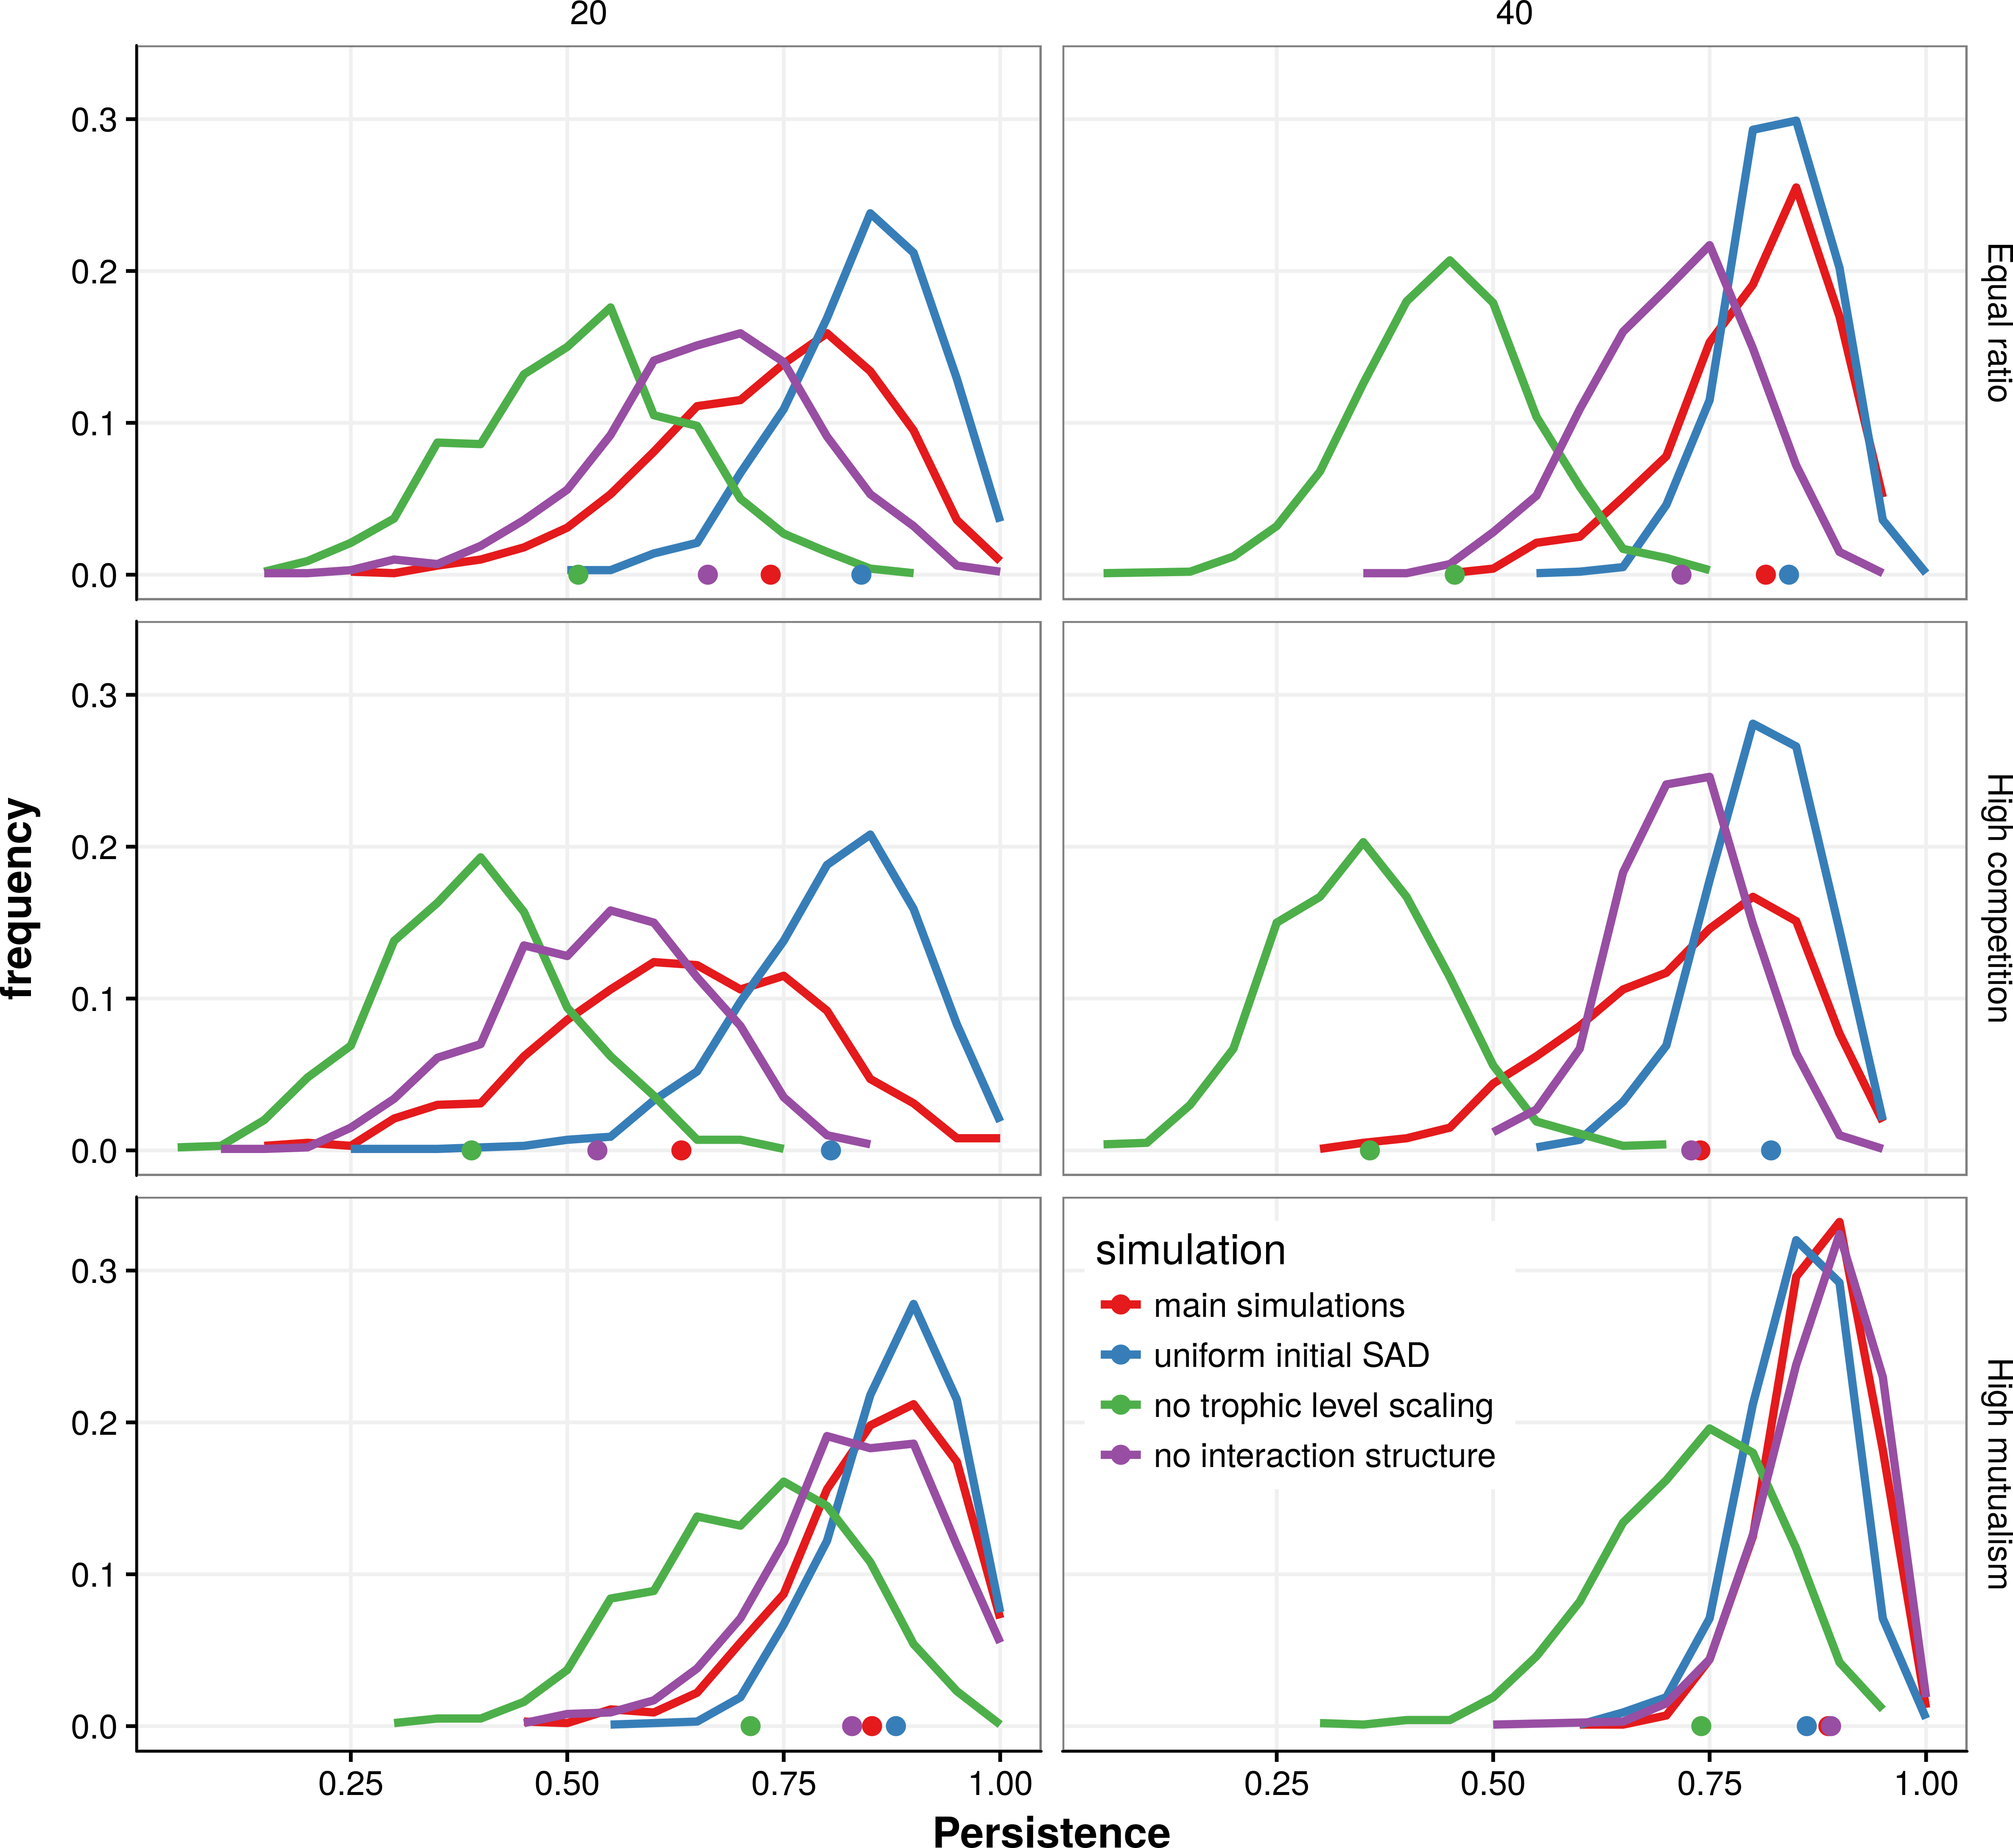
\includegraphics[width=\textwidth]{./Figures/Appendix3_3/Fig_1.png}
\caption[Persistence levels of additional simulations]{\color{Gray} Persistence ratios of the additional simulations. C.f. \cref{fig:fig3.2} of Chapter 3.}
\label{fig:figApp3.3.1}
\end{figure}

\begin{figure}[!htb]
\centering
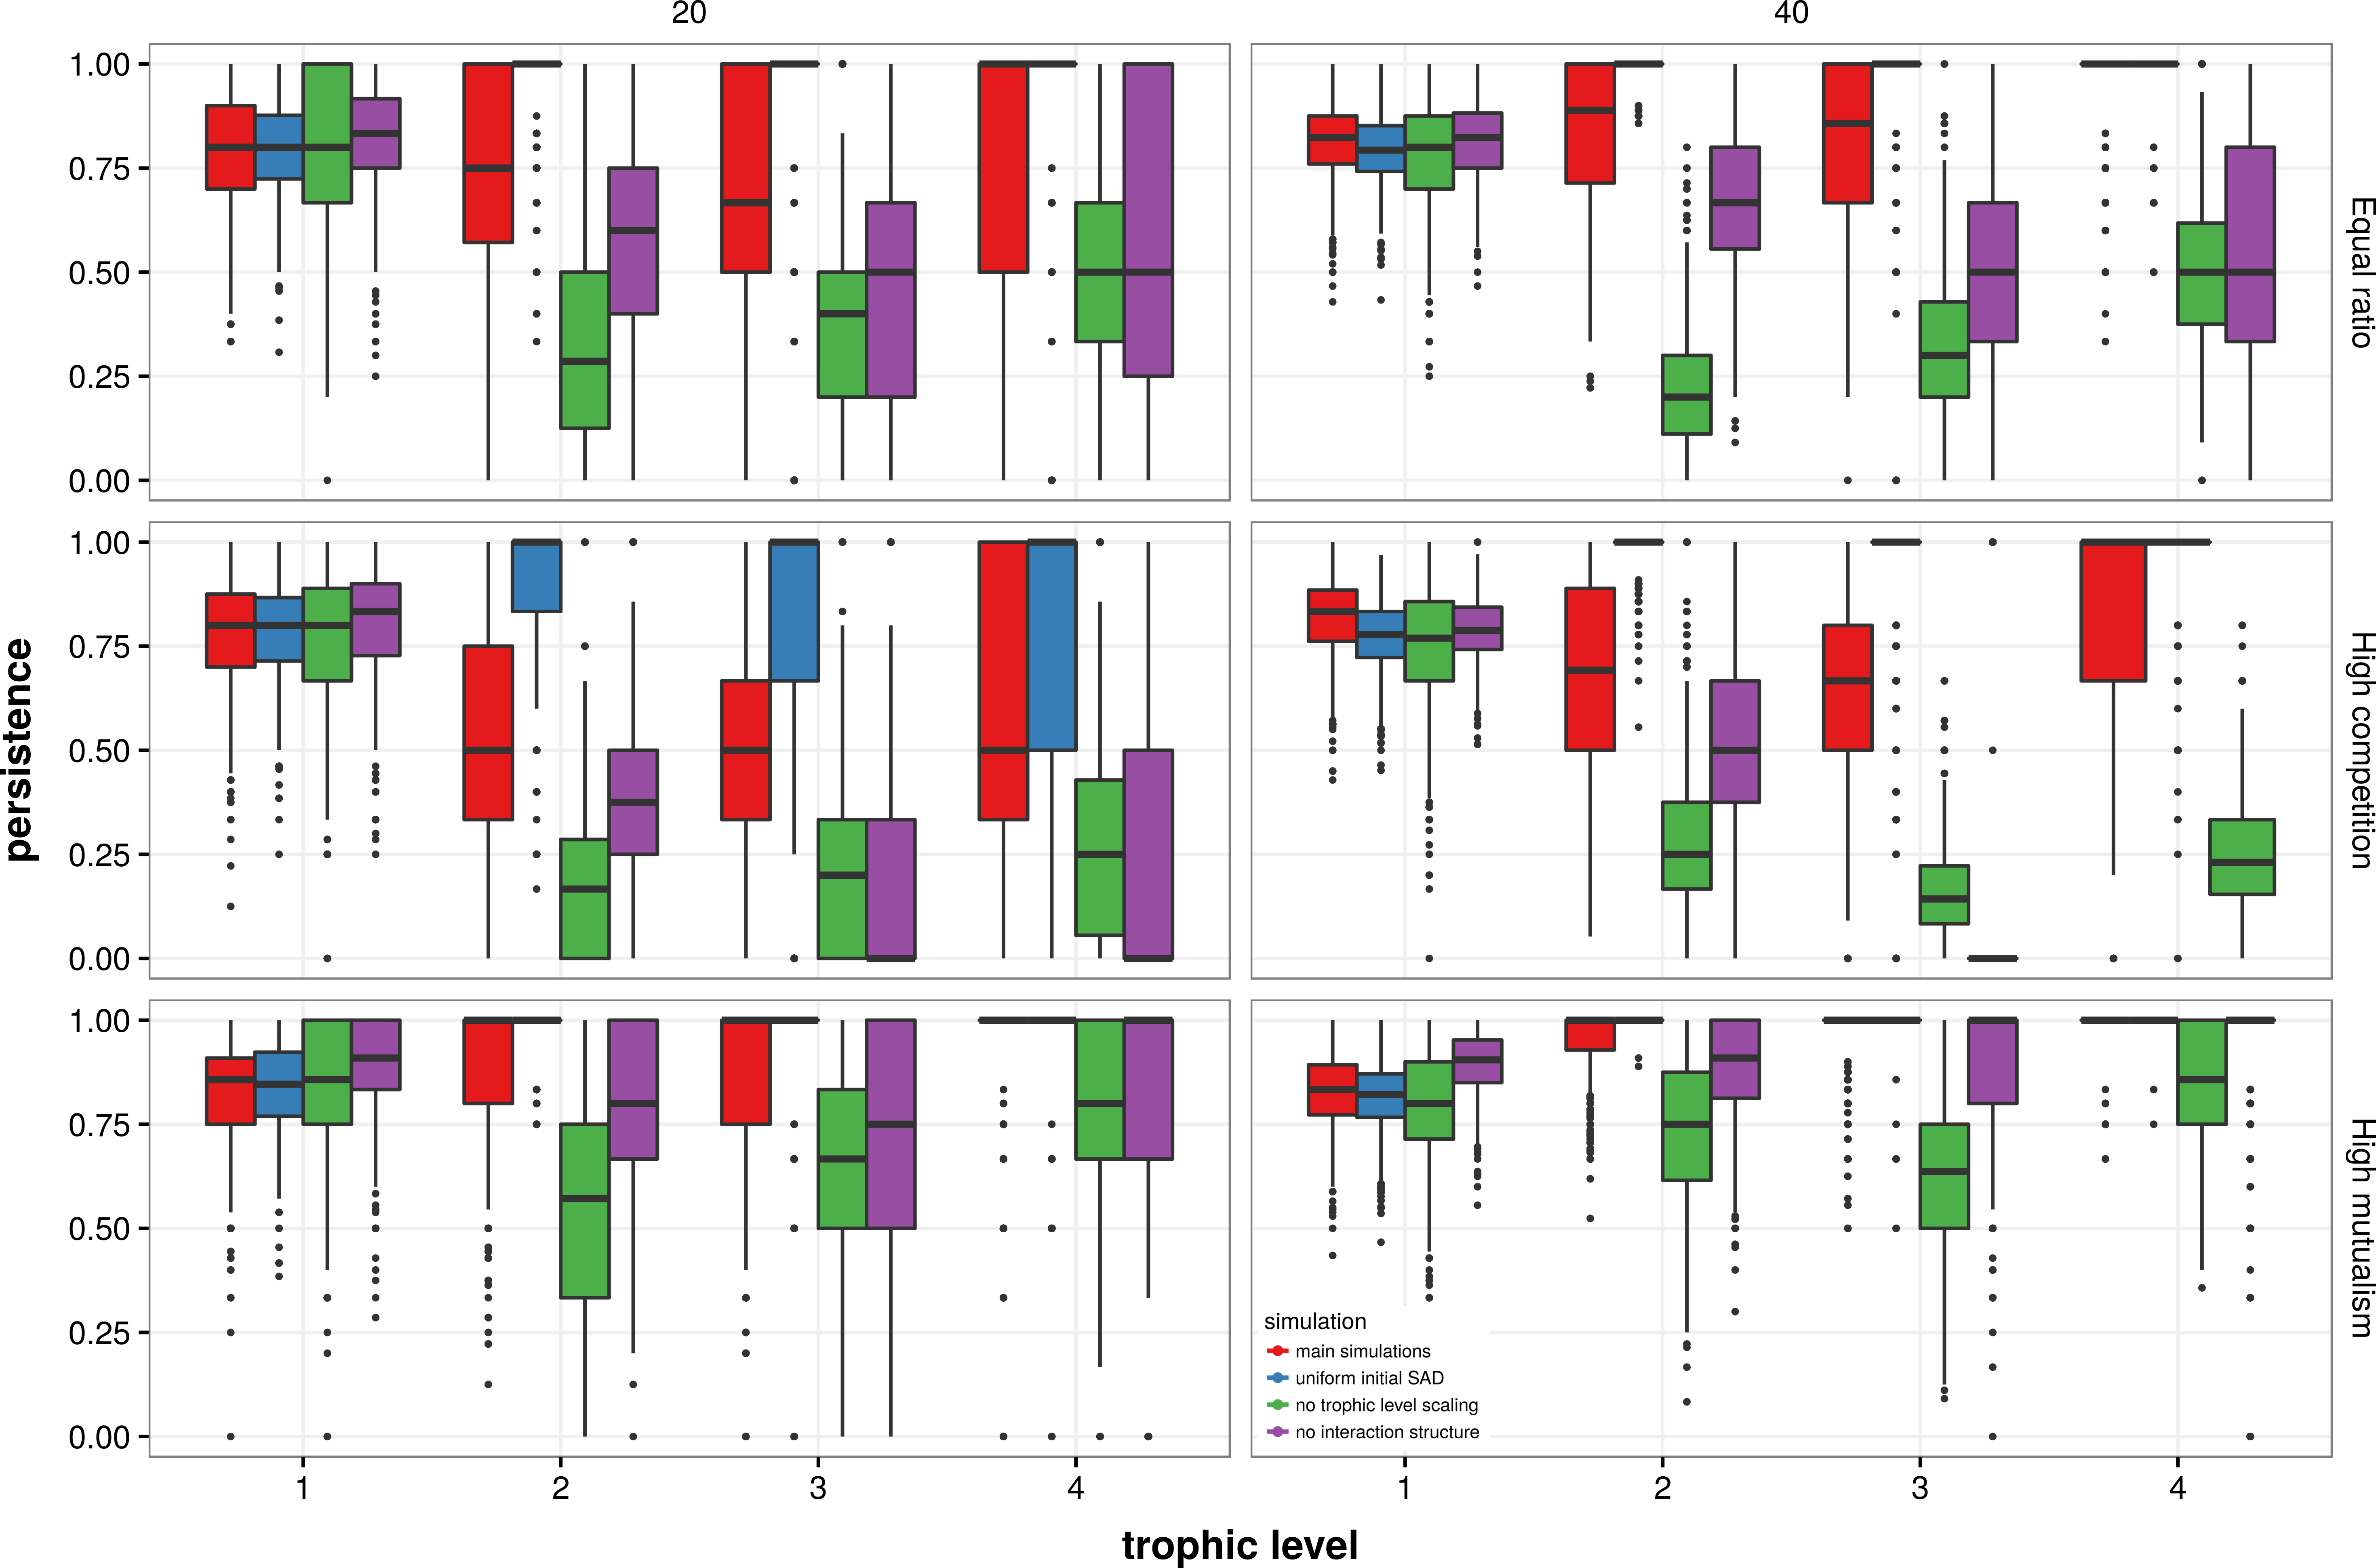
\includegraphics[width=\textwidth]{./Figures/Appendix3_3/Fig_2.png}
\caption[Persistence levels of additional simulations by trophic level]{\color{Gray} Persistence ratios of the four different trophic levels for the additional simulations. C.f. Appendix 3.2: \cref{fig:figApp3.2.1}}
\label{fig:figApp3.3.2}
\end{figure}

\newpage

\begin{figure}[!htb]
\centering
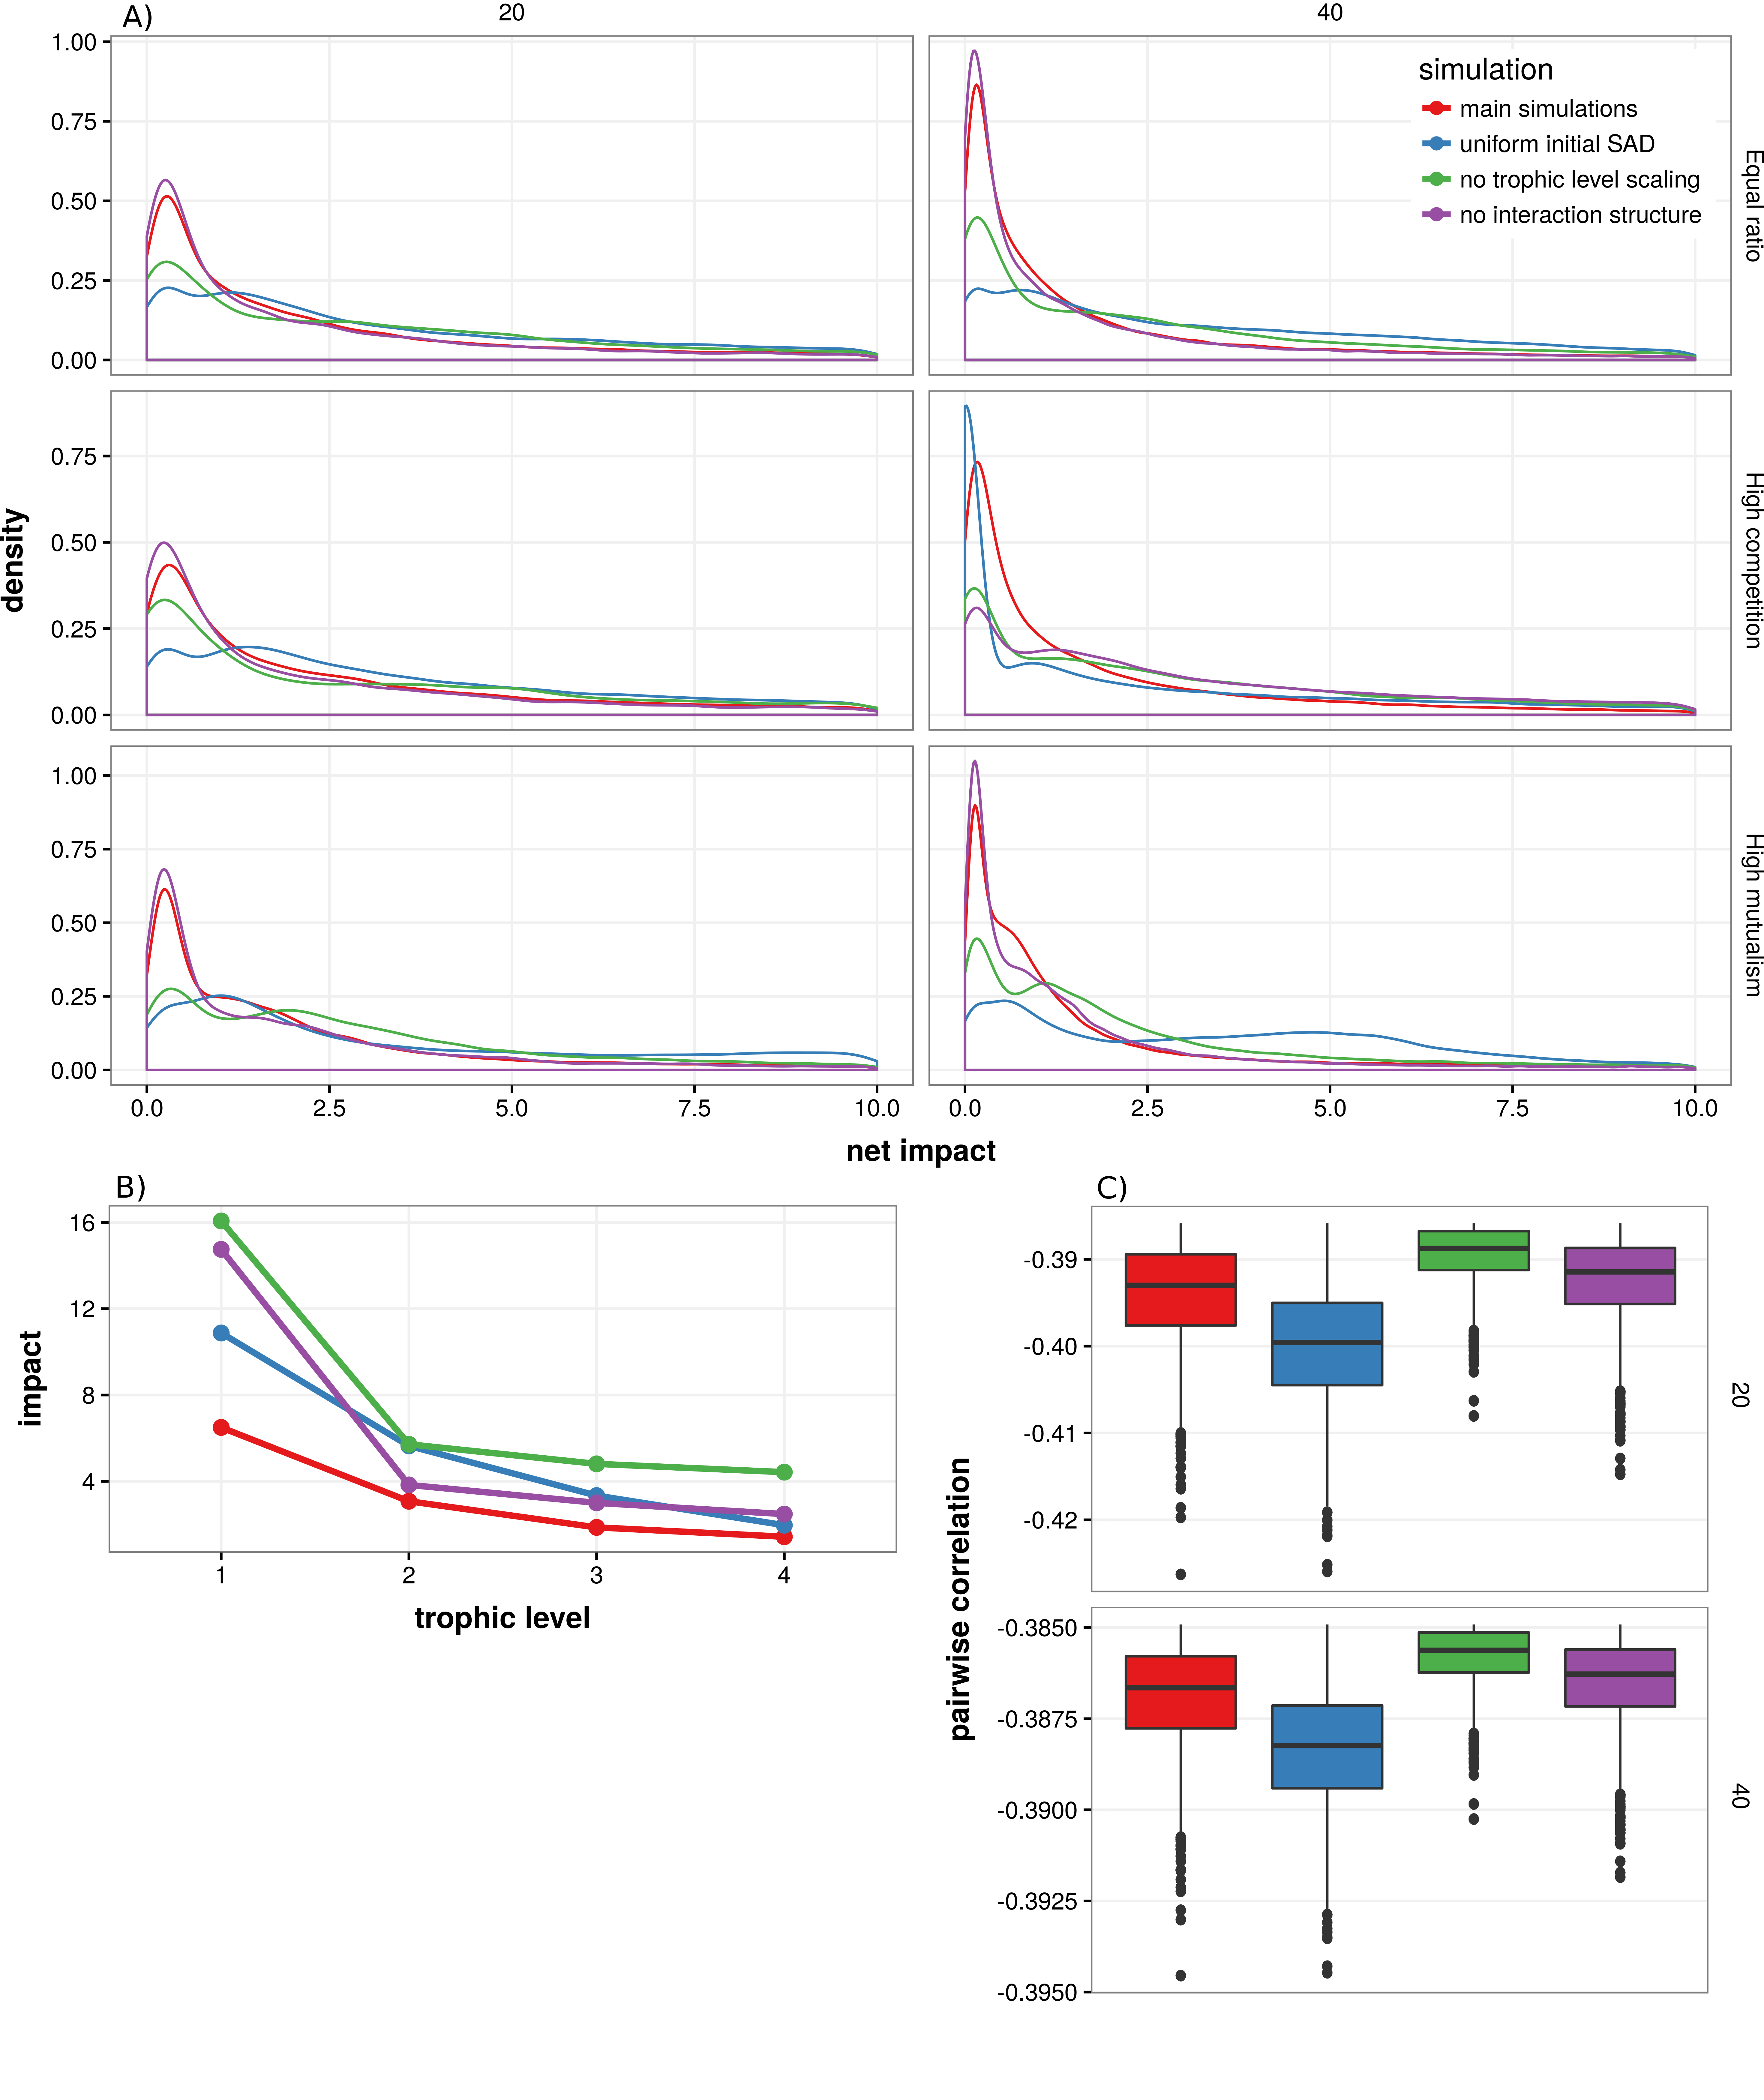
\includegraphics[width=\textwidth]{./Figures/Appendix3_3/Fig_3.png}
\caption[Impact patterns of the additional simulations]{\color{Gray} Species impact and correlation patterns at the end of the additional simulations. C.f. \cref{fig:fig3.3} of Chapter 3.}
\label{fig:figApp3.3.3}
\end{figure}

\newpage

\section*{Sensitivity analysis}

We performed a partial sensitivity analysis on one of the parameters of the model in order to test its qualitative trends. The parameter selected is the scale factor $k$, that modulates the relative scale of a given per capita interaction: a higher k implies a higher per capita impact, up to the point that \(k = 1\) produces per capita interactions that have the same order of magnitude as the intrinsic growth rates.

The motivation behind this parameter is to differentiate interactions by their per capita impact. For example, a single predator-prey interaction will generally have a higher per capita impact than any other single interaction, due to the death of the prey individual. Of course, there are exceptions to this scheme, so we checked the behaviour of our model by producing a small set of simulations with varying sets of k values.

A set of $k$ values specifies the scaling factor for each of the five interaction types, e.g.:

\[k = (k_{amensalism}, k_{antagonism}, k_{commensalism}, k_{competition}, k_{mutualism})\]

The main simulations represent the hypothesis stated above, i.e. that antagonisms will generally have a higher per capita impact:

\[k_{main} = (0.1,0.5,0.1,0.1,0.1)\]

We generated three more sets of $k$ values for this sensitivity analysis, thus obtaining a gradient from complete homogeneity in per capita impact (\(k_1\)) to the initial parameterization (\(k_4\)):

\begin{align*}
& k_1 = (0.2,0.2,0.2,0.2,0.2)\\
& k_2 = (0.167,0.3,0.167,0.167,0.167)\\
& k_3 = (0.133,0.4,0.133,0.133,0.133)\\
& k_4 = k_{main}
\end{align*}

We tested the effect of the different sets of \(k\) in the dynamics of model communities with 20 species and three different configurations of interaction frequencies: an equal ratio of interactions, a high ratio of competition, and a high ratio of mutualism. We generated 500 replicates of each combination of initial richness, interaction frequencies and set of \(k\) values. Computational constraints prevented us from testing the effect of \(k\) over the complete set of community configurations, but the categories selected are representative of the whole set: communities with 20 species are, as shown in e.g. \ref{fig:fig3.2}, the most sensitive to variations in the model parameters; in addition, the three configurations of interaction frequencies selected represent two extremes and an intermediate situation in regards to expected persistence. Therefore, we are moderately confident that the results from this sensitivity analysis can be representative of other configurations.

The results of the sensitivity analysis show that homogeneous \(k\) values across interaction types tend to increase persistence levels, for every configuration, and the differences between configurations are statistically significant in most cases (Fig. \ref{fig:figApp3.3.4}). Statistical comparisons across groups were analyzed by performing Bonferroni-corrected pairwise Wilcoxon signed-rank tests on each pair of persistence values. It is also apparent that, regardless the set of \(k\) values chosen, communities with high proportion of mutualisms show the highest levels of persistence, while communities with high proportion of competition show the lowest levels. Therefore, the qualitative trends of the main simulations are maintained across different sets of interaction scaling factors.

\begin{figure}[!ht]
\centering
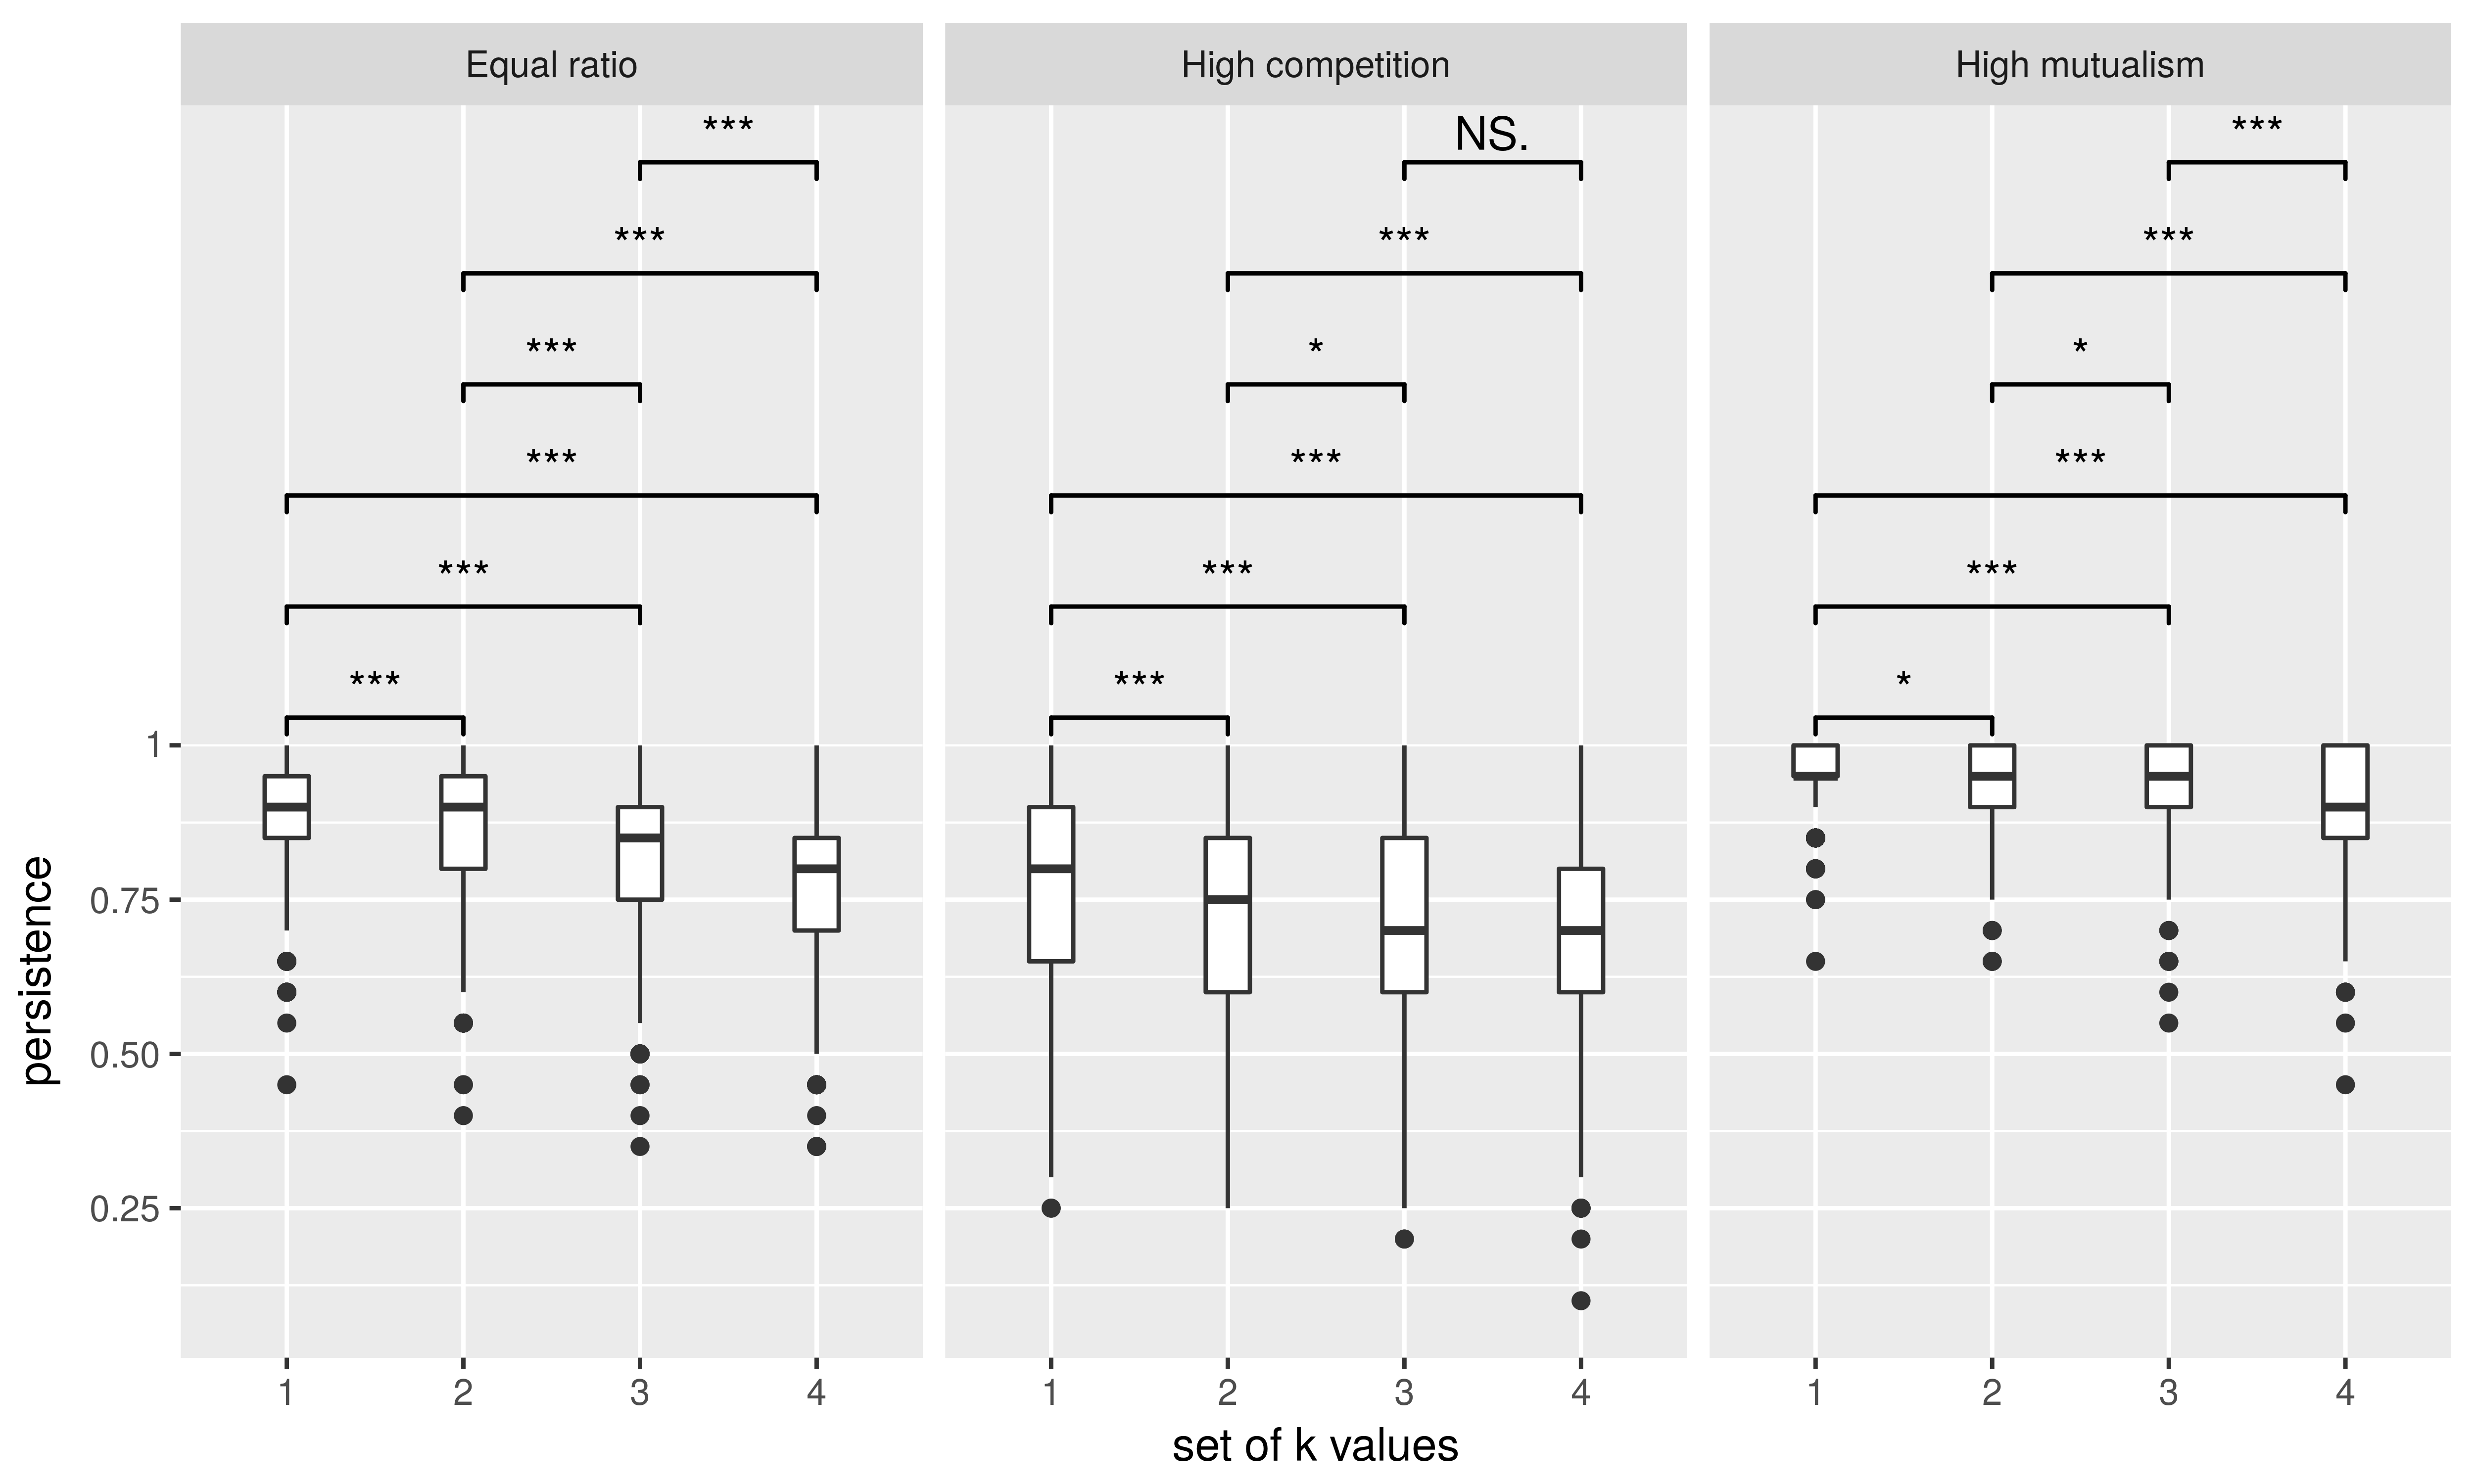
\includegraphics[width=\textwidth]{./Figures/Appendix3_3/Fig_4.png}
\caption[Sensitivity analysis]{\color{Gray} Distribution of persistence values for 500 replicates of model communities parameterized with different sets of values for the scaling factor \(k\). The x axis represents the different sets of values considered (see text). Bars above the boxplot represent the significance of each pairwise comparison (Wilcoxon signed-rank tests; * indicates p \textless{} 0.05, ** p \textless{} 0.01, *** p \textless{} 0.001}
\label{fig:figApp3.3.4}
\end{figure}
